\section{Results}
\label{sec:results}

\subsection{vs. MultiASR}
\label{ssec:baseline-multitask}

As presented in Table \ref{tab:llp-table} and \ref {tab:flp-table}, compared to monolingual training (without using pretrained weights as initialization,  listed on the first row of table and denoted as no-pretrain), MultiASR and MetaASR showed that multilingual pretraining using different combinations of source languages can improve ASR performance on target language. Besides, the proposed MetaASR significantly outperforms MultiASR across all target languages.
\begin{figure}[ht]
  \centering
  %\hspace{-2.2cm}
  \begin{tikzpicture}[trim axis left, trim axis right]

  \begin{axis}[
    width=\linewidth,
    %height=7.5cm,
    legend entries={MultiASR, MetaASR, no-pretrain} ,
    xlabel = {Number of pretraining steps ($\times 1000$)},
        xmin=5,
        %xmax=130,
        %ymax=71,
        grid=both,
        legend style={at={(0.02,0.74)},anchor=north west},
        %legend pos=outer north east,
        ylabel={CER (\si{\percent}})]
  \addplot+[smooth]table{multi-stat/multi3-swahili};
  \addplot+[smooth]table{meta-stat/meta3-swahili};
   \addplot[style=ultra thick,dashed,] coordinates {(0,64.3) (100,64.3)};
   %\addplot[style=ultra thick,dashed, gray] coordinates {(0,0.589) (200,0.589)};
   %\addplot[style=ultra thick,dashed, brown] coordinates {(0,0.628) (200,0.628)};
  \end{axis}
  \end{tikzpicture}
  %\caption{Pretrain on EN, FI, FR, NL, RM, RU, and evaluate on }
  \caption{Learning curves on Swahili's LLP \\ pretrained on Bn, Tl, Zu}
  \label{fig:curve1}
  \vspace{-10pt}
\end{figure}


\begin{figure}[ht]
  \centering
  %\hspace{-2.2cm}
  \begin{tikzpicture}[trim axis left, trim axis right]

  \begin{axis}[
    width=\linewidth,
    height=6.5cm,
    %legend entries={MultiASR, MetaASR} ,
    legend entries={MultiASR, MetaASR, no-pretrain} ,
    xlabel = {Number of pretraining steps ($\times 1000$)},
        xmin=5,
        %xmax=130,
        grid=both,
        legend style={at={(0.02,0.48)},anchor=south west},
        %legend pos=inner north west,
        ylabel={CER (\si{\percent}})]
  \addplot+[smooth]table{multi-stat/multi6-swahili};
  \addplot+[smooth]table{meta-stat/meta6-swahili};
   \addplot[style=ultra thick,dashed,] coordinates {(0,64.3) (100,64.3)};
   %\addplot[style=ultra thick,dashed, gray] coordinates {(0,0.589) (200,0.589)};
   %\addplot[style=ultra thick,dashed, brown] coordinates {(0,0.628) (200,0.628)};
  \end{axis}
  \end{tikzpicture}
  %\caption{Pretrain on EN, FI, FR, NL, RM, RU, and evaluate on }
  \center \caption{Learning curves on Swahili's LLP \\  pretrained on Bn, Tl, Zu, Tr, Lt, Gn}
  \label{fig:curve2}
  \vspace{-10pt}
\end{figure}

% Hsu: (TODO) 等 final evaluation 出來後,會再加上幾句話



\subsection{Training Curves}
% (TODO) 等 FLP 跑出來後,看一下 overfitting 是否比較沒那麼嚴重,可以再加幾句話
% ,不然就是再補不同的圖,說這個現象很普遍 (的確也是)

The advantage over MetaASR over MultiASR is clearly shown in Fig. \ref{fig:curve1} and \ref{fig:curve2}. For MultiASR, the performance of adaptation saturates in early stage and finally degrades. As Fig. \ref{fig:meta-idea} illustrated, the training scheme of MultiASR tends to overfit on source languages, thus the learnt parameter may not be suitable for adaptation. In contrast, for MetaASR, not only the performance is better than MultiASR during whole pretraining process, but also gradually improves as pretraining continues without degrading.


\subsection{Training Set Size}
\textcolor{red}{(TBD)} Depend on final evaluation \textcolor{red}{(TBD)}
%% ref: http://pgfplots.net/tikz/examples/bar-plot/
\begin{figure}[t]
\begin{minipage}[b]{1.0\linewidth}
    \raggedright
    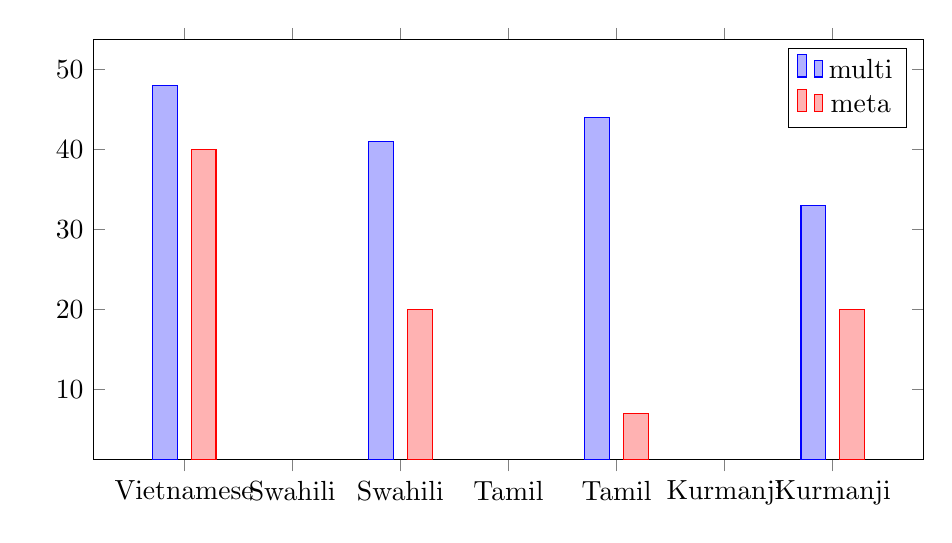
\begin{tikzpicture}
\begin{axis}[
	x tick label style={
		/pgf/number format/1000 sep=},
    ylabel= {\si{\percent}},
	enlargelimits=0.14,
	symbolic x coords={Vietnamese,Swahili,Tamil,Kurmanji},
	xticklabel style={align=center},
	ybar=5pt,
	height=.57\textwidth,
	width=\textwidth,
	bar width=9pt,
]

\addplot 
	coordinates {(Vietnamese,48) (Swahili,41)
		 (Tamil,44) (Kurmanji,33) };

\addplot 
	coordinates {(Vietnamese,40) (Swahili,20) 
		(Tamil,7) (Kurmanji,20) };

\legend{multi, meta}
\end{axis}
\end{tikzpicture}
\caption{CER relative improvement from LLP to FLP \textcolor{red}{Waiting for stat}}
    \label{fig:impact-on-size}
\end{minipage}

\end{figure}

%\label{ssec:training-size}
%Fig. \ref{fig:impact-on-size},
%If Meta and Multi achieve nearly the same performance in FLP(which is the case in MetaNMT), we want to see Meta can achieve better in LLP (so the lower the bar of meta, the better )
